
\section{Impulse, Momentum, and Interactions\footnote{
1990-93 Dept. of Physics and Astronomy, Dickinson College. Supported by FIPSE
(U.S. Dept. of Ed.) and NSF. Portions of this material may have been modified
locally and may not have been classroom tested at Dickinson College.
}}

Name \rule{2.0in}{0.1pt}\hfill{}Section \rule{1.0in}{0.1pt}\hfill{}Date \rule{1.0in}{0.1pt}

\textbf{Objectives }

\begin{itemize}
\item To verify the relationship between impulse and momentum experimentally. 
\item To study the forces between objects that undergo collisions and other types of interactions in a short time period.
\end{itemize}
\textbf{Apparatus} 

\begin{center}
\begin{tabular}{|l|l|l|} \hline
Dynamics cart with flag and track   & Force probe   & Motion sensor \\ \hline
{\it Science Workshop 750 Interface}& compact scale & {\it DataStudio} \\ \hline
\end{tabular}
\end{center}

\textbf{The Impulse-Momentum Theorem }

Real collisions, like those between eggs and hands, a Nerfball and a wall, or
a falling ball and a table top are tricky to study because $\Delta t$ 
is so small and
the collision forces are not really constant over the time the colliding objects
are in contact. Thus, we cannot calculate the impulse as $F \,\Delta t$. 
Before we study
more realistic collision processes, let's redo the theory for a variable force.
In a collision, according to Newton's second law, the force exerted on a falling
ball by the table top at any infinitesimally small instant in time is given
by
\[
{\bf F}=\frac{d{\bf p}}{dt}\qquad [Eq.\: 1]\]


To describe a general collision that takes place between an initial time \( t_{i} \)
and a final time \( t_{f} \) , we must take the integral of both sides of the
equation with respect to time. This gives
\[
\int _{t_{i}}^{t_{f}}{\bf F}dt=\int _{t_{i}}^{t_{f}}\frac{d{\bf p}}{dt}dt=\left( {{\bf p}_{f}}-{{\bf p}_{i}}\right) =\Delta {\bf p}\qquad [Eq.\: 2]\]


Impulse is a vector quantity defined by the equation
\[
{\bf I}=\int_{t_{i}}^{t_{f}}{\bf F}\,dt\qquad [Eq.\: 3]\]


By combining equations {[}2{]} and {[}3{]} we can formulate the impulse-momentum
theorem in which
\[
{\bf I}=\Delta {\bf p}\qquad [Eq.\: 4]\]


If you are not used to mathematical integrals and how to solve them yet, don't
panic. If you have a fairly smooth graph of how the force $F$ varies as a function
of time, the impulse integral can be calculated as the area under the $F$-$t$ 
curve.

Let's see qualitatively what an impulse curve might look like in a real collision
in which the forces change over time during the collision. In particular, let's
consider the collision of a Nerfball with a wall as shown below.

\vspace{0.3cm}
{\par\centering 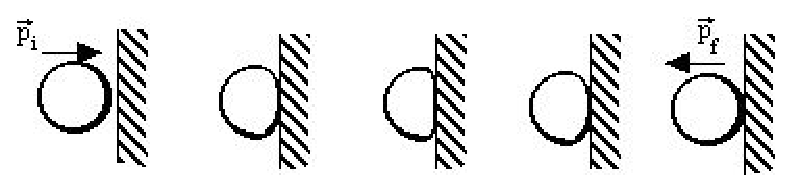
\includegraphics{impulse/impulse_fig1.eps} \par}
\vspace{0.3cm}

\textbf{Activity  \stepcounter{activity}\arabic{activity}: Predicting Collision Forces That Change }

(a) Suppose a tennis ball is barreling toward a wall and collides with it. If friction is neglected, what is the net force exerted on the object just before it starts to collide?
\vspace{10mm}

(b) When will the magnitude of the force on the ball be a maximum? 
\vspace{10mm}

(c) Roughly how long does the collision process take? Half a second? Less? Several
seconds?
\vspace{10mm}

(d) Attempt a rough sketch of the shape of the force the wall exerts on a moving
object during a collision.

\vspace{0.3cm}
{\par\centering 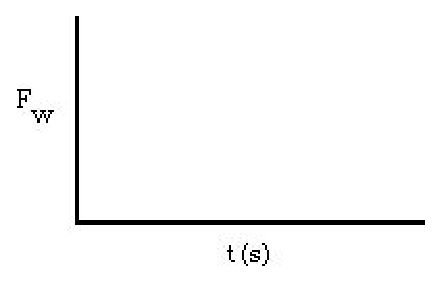
\includegraphics{impulse/impulse_fig2.eps} \par}
\vspace{0.3cm}

\textbf{Verification of the Impulse-Momentum Theorem} 

To verify the impulse-momentum theorem experimentally we must show that for
an actual collision involving a single force on an object the equation
\[
\int_{t_{i}}^{t_{f}}{\bf F}\,dt=\Delta {\bf p}\]


holds, where the impulse integral can be calculated by finding the area under
the curve of a graph of $F$ vs. $t$.

\vspace{0.3cm}
{\par\centering 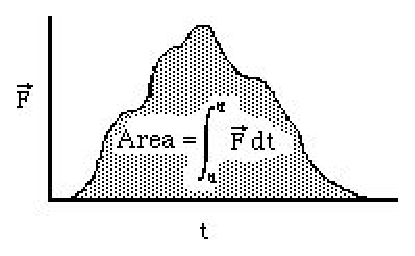
\includegraphics{impulse/impulse_fig3.eps} \par}
\vspace{0.3cm}

In this experiment you will investigate this theorem by measuring the impulse
and the change in momentum of a cart undergoing a one-dimensional collision.
The experimental setup is shown in the figure below. The end of the track with
the motion detector should be raised about 1.5 cm so that, when released, the
cart will collide with the force probe. The force probe will measure the force
as a function of time during the collision. The motion detector is used to measure
the velocity of the glider before and after the collision. You will use the
Impulse-Momentum application to make these measurements.

\vspace{0.3cm}
{\par\centering \resizebox*{0.9\textwidth}{!}{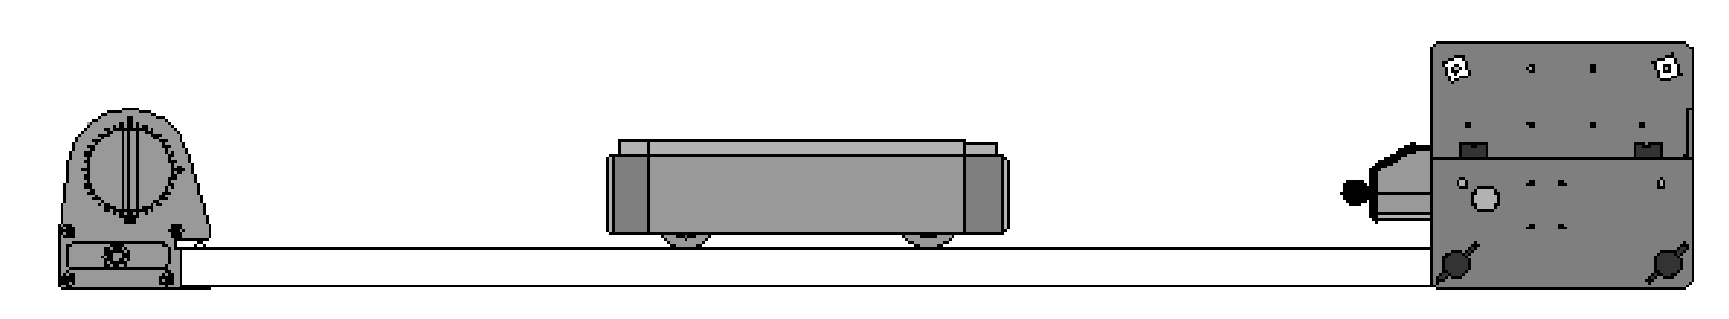
\includegraphics{impulse/impulse_fig4.eps}} \par}
\vspace{0.3cm}

\textbf{Activity  \stepcounter{activity}\arabic{activity}: Verification of the Impulse-Momentum Theorem} 

(a) Measure and record the mass of the cart, $m$, using the compact scale.
\vspace{10mm}

(b) Calibrate the force probe (see \textit{Calibrating Force Sensors} in \textbf{Appendix E: Instrumentation}). \textbf{NOTE:} The force probe must be removed from its bracket and the rubber bumper replaced by a hook so that the force probe can be held VERTICALLY for the calibration. After calibrating, return the rubber bumper to the force probe, attach the force probe to its bracket, and close V, A \& F Graphs Application.

(c) Construct a data table in the space below with the column headings Trial
\#, Area, \( v_{i} \), and \( v_{f} \). Make enough room to record seven trials.

\begin{center}
\begin{tabular}{|p{1.0in}|p{1.0in}|p{1.0in}|p{1.0in}|} \hline
 & & & \\ \hline
 & & & \\
 & & & \\
 & & & \\
 & & & \\
 & & & \\
 & & & \\
 & & & \\
 & & & \\
 & & & \\
 & & & \\
 & & & \\
 & & & \\
 & & & \\ \hline
\end{tabular}
\end{center}

(d) Position the force probe part way up the track (to be closer to the motion sensor). Open the \textbf{Impulse-Momentum} application in the \textbf{131 Workshop} submenu. 

(e) Set the cart on the track about mid-way between the motion sensor and the force probe. Start recording data and release the cart. Stop recording data after the cart collides with the force probe and bounces back. The computer will then display graphs of velocity and force versus time.

(f) Determine the area under the force vs. time graph and record the value in
your data table. See \textbf{Appendix B: Introduction to DataStudio} for instructions on how to determine the area under a curve.

(g) Use the smart tool to find the velocity just before the collision and the
velocity just after the collision from the velocity versus time graph. Record
these values in your data table.

(h) Repeat parts (e) through (g). For these trials, 
the area function and the smart tool must be turned on and off for each trial. 
Print the graphs for one of your trials and include it with this report.

\newpage

(i) Construct another data table below with the column headings
Trial \#, $I$, \( \Delta  p\), Diff., and Percent diff. For each trial, calculate and record
the impulse, $I$, and the change in momentum, \( \Delta  p\), in kg\,m/s. Also,
determine the difference between $I$ and $\Delta p$  for each trial, and the percent difference. Also, show a sample
calculation of $I$ and \( \Delta  p\) for one of your trials.

\begin{center}
\begin{tabular}{|p{1.0in}|p{1.0in}|p{1.0in}|p{1.0in}|p{1.0in}|} \hline
 & & & & \\ \hline
 & & & & \\
 & & & & \\
 & & & & \\
 & & & & \\
 & & & & \\
 & & & & \\
 & & & & \\
 & & & & \\
 & & & & \\
 & & & & \\
 & & & & \\
 & & & & \\
 & & & & \\ \hline
\end{tabular}
\end{center}

(j) What do you expect for the values in the last column of your table (Percent diff)? Make a histogram of your results in that column and calculate the average and standard deviation. For information on making histograms, see \textbf{Appendix C}. For information on calculating the average and standard deviation, see \textbf{Appendix A}. Record the average and standard deviation here.
Attach the histogram to this unit.
Is your data consistent with your expectation?  Be quantitative in your answer.
\vspace{20mm}

(k) Do your results verify the impulse-momentum theorem? Explain quantitatively.
\vspace{20mm}

(l) What does the histogram of your data tell you? Be quantitative in your answer.
\vspace{20mm}

(m) Is there any indication of a systematic uncertainty? What are the possible
sources of error?

